\documentclass[12pt,a4paper,oneside]{report}
\usepackage[utf8]{inputenc}
\usepackage[english]{babel}
\usepackage{amsmath}
\usepackage{amsfonts}
\usepackage{amssymb}
\usepackage{graphicx}
\usepackage[left=3cm,right=2cm,top=3cm,bottom=2cm]{geometry}
\begin{document}

\begin{center}
\textbf{\large{Context Description and Next Activities}}
\end{center}
\bigskip

\begin{figure}[b!]
\center
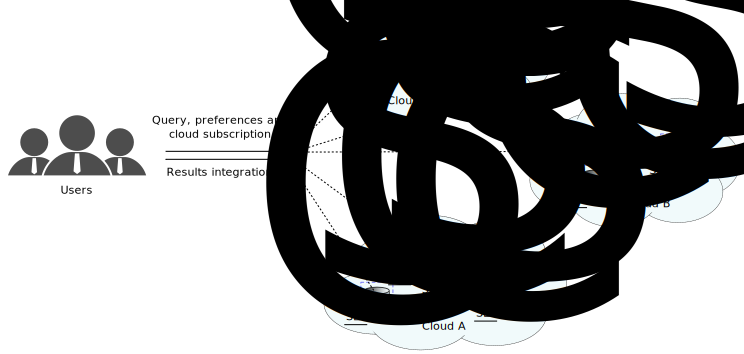
\includegraphics[scale=1]{figures/scenario.pdf}\caption{Data integration context overview}\label{fig:context}
\end{figure}

The figure~\ref{fig:context} illustrates our data integration scenario. Cloud providers (for instance, Data Provider A, Data Provider B and Data Provider C) offer cloud services to data services (for instance, Data service 1, Data service 2, Data service 3 and Data service 4) willing to deploy their services. The cloud provider and the data service establish a contract specifying what guarantees in terms of infrastructure resources (for instance, storage limit, memory limit, processing capacity) the data service can expect from the cloud. This contract is called \textsl{Cloud SLA} ($SLA_{C}$).

Data services can deploy services in the clouds they have subscriptions respecting what is agreed in the $SLA_{C}$. Each service deployed by the data service in the cloud export a different SLA (called \textsl{Service SLA} - $SLA_{S}$) which specifies what service customers can expect in terms of data quality guarantees (for instance, provenance, freshness, data type, degree of rawness) from its service. The data service defines the $SLA_{S}$ according to what it is defined in the $SLA_{C}$. In other words, the $SLA_{S}$ is derived from the $SLA_{C}$. Moreover, a data service can deploy the same service in different clouds in which it has established contracts (for instance, the Data service 1 deployed the service S1 in the cloud provider A and B) and for each different cloud provider different $SLA_{S}$ are defined for the same service.

The end-user willing to integrate data interacts with our \textsl{Data Integration-as-a-Service} (\textsl{DIaaS}). The \textsl{DIaaS} is responsible to select and match the services that can produce the result expected by the user according to his preferences, where he is consuming the data, and the different SLAs associated to the services and to the cloud providers. Once the composition is created and executed, the integration results are delivered to the user and an \textsl{integration SLA} ($SLA_{I}$) established. This SLA is responsible to include information collected during the integration process which can be reused in a further integration request.

\paragraph{Activities for the next meeting:}
\begin{enumerate}
\item Enumerate the possible cases of queries and their variations to be able to identify what could be interest to be in the \textsl{integration SLA} and what information should I collect in the integration process.
\item Propose the schemas of $SLA_{C}$ and $SLA_{S}$ according to the schema that I have removing what is not necessary for it.
\end{enumerate}

\end{document}